\chapter{Revisão de literatura}
\label{cap:revisao-literatura}

Este capítulo revisa estudos relacionados aos temas do trabalho: a evolução dos modelos preditivos, o PIB, o uso desses modelos para variáveis macroeconômicas e os critérios empregados em sua comparação.

Esta revisão começa pela previsão econômica e pelo \ac{pib}, variável de interesse do estudo. Em seguida, apresenta os modelos econométricos tradicionais e os modelos baseados em IA selecionados, com seus conceitos, características e aplicações à previsão de variáveis econômicas. A discussão de estudos anteriores acompanha a apresentação de cada modelo.

%\section{Estudos Anteriores}
\section{Previsão econômica e PIB}

% BC CVM FEBRABAM

A previsão de variáveis econômicas não é recente. Desde o início do século XX, economistas buscam descrever o comportamento dessas variáveis ao longo do tempo. Em seu artigo, \citeonline{FrischSTATIKKOD} apresenta uma teoria dinâmica dividida em duas vertentes: a analítica, que trata das leis que regem as flutuações das variáveis, e a histórica, que aplica essas leis para descrevê-las e prevê-las. Essa distinção contribuiu para o desenvolvimento posterior da econometria e de suas aplicações.

Segundo \citeonline{almeida_2001}, no início do século XX, a economia passou por uma fase madura de industrialização e incorporou numerosas inovações tecnológicas decorrentes da Segunda Revolução Industrial. O autor afirma que "a estrutura da produção foi radicalmente transformada pelas mudanças introduzidas nos padrões de trabalho (especialização) e pelos avanços tecnológicos, que aumentaram dramaticamente o produto per capita" \citem[p. 2]{almeida_2001}.

Segundo \citeonline{junior_2017}, a Terceira Revolução Industrial também promoveu mudanças na atividade produtiva. O autor ressalta que essa transformação não ocorreu de forma homogênea e foi marcada por uma revolução técnico-científica que alcançou não apenas as fábricas, mas também diversas atividades socioeconômicas. Além disso, alguns autores identificam uma nova etapa, denominada Quarta Revolução Industrial ou Indústria 4.0.
% Citar autor que confirma a complexidade da economia

O termo Indústria 4.0 foi apresentado na feira de Hannover como parte de uma política alemã de industrialização \citem{kagermann2013recommendations}. A Indústria 4.0 corresponde à transformação digital da indústria, que integra tecnologias como a inteligência artificial. \citeonline{martins2021industria} discute essa etapa industrial e as mudanças associadas a ela, como a criação de novos modelos de negócio e o surgimento de mercados mais exigentes.

Além de transformar a atividade produtiva, a Indústria 4.0 ampliou as possibilidades de coleta e processamento de grandes volumes de dados por meio dos sistemas de informação.
% Trazer algum autor sobre a industria 4.0
Segundo \citeonline{laudon2022sistemas}, esses sistemas são essenciais para que as organizações alcancem seus objetivos estratégicos. As informações geradas podem subsidiar decisões nos setores público e privado.
%	Na era digital, o grande volume de dados gerados pelos sistemas de informação pode ser usada como uma fonte, praticamente inesgotável de informações para tomadas de decisões. 

\begin{citacao}
	A eficácia das políticas depende do uso de todas as informações disponíveis em qualquer momento, incluindo informações prospectivas, como desempenho do mercado de ações e a incerteza da política econômica, disponíveis no ponto de estimativa. \citem[p. 19]{ghosh2023machine}
\end{citacao}

A análise econômica utiliza indicadores microeconômicos, relacionados às firmas, e indicadores macroeconômicos, voltados aos grandes agregados. Entre estes, destaca-se o \ac{pib}, que sintetiza a produção de bens e serviços finais de uma economia. Segundo o \ac{ibge}, "o \ac{pib} é a soma de todos os bens e serviços finais produzidos por um país, estado ou cidade, geralmente em um ano" \citem[p. 1]{ibge_pib}.

O Banco Central do Brasil define o PIB a preços de mercado como o total de bens e serviços produzidos pelas unidades produtoras residentes e destinados ao consumo final, excluído o consumo intermediário \citem[p. 1]{BCB_SGS_1207}. A série 1207 do Sistema Gerenciador de Séries Temporais, também citada pelo Banco Central, apresenta o PIB em reais correntes: os valores são calculados a preços do próprio período, sem descontar as variações de preços, o que caracteriza uma medida nominal \citeonline{BCB_SGS_1207}. Para comparar a produção entre períodos sem o efeito das variações de preços, utilizam-se medidas de volume ou valores constantes. Neste trabalho, analisa-se o PIB real brasileiro, tanto em nível quanto em taxa de crescimento, com frequência anual.

A definição de PIB apresentada pelo \ac{bea} é compatível com as do Banco Central do Brasil e do \ac{ibge}. Segundo o \citeonline{BEA_GDP}, o PIB mede o valor dos bens e serviços finais produzidos, excluídos os bens e serviços intermediários. O \ac{bea} também destaca a relevância do indicador: "as mudanças no PIB são o indicador mais popular da saúde econômica geral do país" \citem[p. 1]{BEA_GDP}.

% Professor adicionei o conceito do IBGE, do Banco Central e do BEA dos EUA

Nesse sentido, o \ac{pib} funciona como um termômetro da atividade econômica. À medida que a economia se transforma e a disponibilidade de dados se amplia, também evoluem os métodos utilizados para analisar e prever o comportamento desse indicador.

% Colocar mais complexidade na definição do PIB

A previsão do PIB é objeto de estudos acadêmicos e também subsidia atividades de instituições públicas e privadas. O \ac{ipea}, por exemplo, destaca sua importância "para a definição dos parâmetros para o planejamento fiscal e orçamentário do setor público, bem como para a formação de expectativas no setor privado" \citem[p. 6]{santos2022previsao}.

A evolução da econometria, a maior disponibilidade de dados e os avanços computacionais ampliaram o conjunto de métodos aplicáveis às previsões econômicas. Nesse contexto, o desempenho relativo dos modelos deve ser avaliado empiricamente para o problema e os dados considerados.
%	Traz um autor sobre modelos tradicionais
%	, conforme .
%	Cabe um Shumpeter aqui

\section{Modelos preditivos}

Antes de apresentar os modelos deste estudo, convém definir o que se entende por modelo preditivo. \citeonline{FrischSTATIKKOD} discute a teoria dinâmica e distingue a análise das leis que regem as flutuações da aplicação dessas leis à descrição e à previsão de variáveis. Como a econometria abrange diferentes tipos de modelos, esta seção delimita o conceito de modelo preditivo e introduz as abordagens examinadas no trabalho.

Para \citeonline[p. 8]{assunccao2012estrategias}, esses modelos "correspondem a uma equação (ou regra) na qual através de informações históricas ou atuais predize-se um determinado evento futuro a respeito de um indivíduo". Aplicada ao problema deste trabalho, essa definição permite distinguir três componentes: as variáveis de entrada, históricas ou contemporâneas; o processamento dessas informações por uma equação matemática ou pelas regras do modelo; e a saída, que corresponde à previsão da variável de interesse para um período futuro.

Com essa definição, retomamos o objetivo deste estudo: prever o PIB real brasileiro em nível e em taxa de crescimento. Nesse caso, os dados de entrada são as variáveis preditoras selecionadas, e a saída é a previsão de um dos alvos definidos. Os modelos também diferem em sua estrutura e na forma como processam as entradas; essas características serão apresentadas nas próximas subseções.

Após a definição dos modelos preditivos, esta seção apresenta os modelos econométricos tradicionais (VAR, ARIMA, DFM e MIDAS) e os dois modelos baseados em IA (redes neurais e Random Forest). Para cada um, são discutidos o conceito, as principais características e as aplicações à previsão do PIB. A exposição começa pelos modelos tradicionais e, em seguida, aborda os modelos de IA.

\subsection{Modelos econométricos tradicionais}

Na bibliografia consultada, "tradicional" aparece como uma classificação comparativa. \citeonline{carmo2023modelagem}, por exemplo, contrapõe a regressão linear, tratada como método clássico, às redes neurais. Neste trabalho, "modelos econométricos tradicionais" designa VAR, ARIMA, DFM e MIDAS, utilizados como métodos econométricos de previsão. Em suas especificações usuais, esses modelos expressam relações lineares, mas se distinguem pela estrutura: o ARIMA é univariado, o VAR é multivariado, o DFM representa fatores dinâmicos e o MIDAS combina dados de frequências distintas. \citeonline[p. 14]{vasconcelos2017poder} caracteriza os modelos lineares pela linearidade da função condicional $E(Y|X)$ nos preditores. Já \citeonline{rebelo2022interpretabilidade} aborda regressão linear e árvores de decisão como modelos de interpretabilidade natural.

Segundo \citeonline{braga2025forecasting}, os modelos tradicionais predominaram por muitos anos na previsão de variáveis econômicas. A autora observa: "Apesar da eficácia desses modelos tradicionais em determinados cenários, os avanços computacionais e a crescente disponibilidade de dados favorecem o desenvolvimento de abordagens mais sofisticadas" \citem[p. 12]{braga2025forecasting}.

Neste estudo, serão abordados quatro modelos econométricos: ARIMA, de natureza univariada; VAR, multivariado; DFM, baseado em fatores dinâmicos; e MIDAS, que permite combinar variáveis observadas em frequências distintas. A seleção busca comparar estruturas distintas de previsão do \ac{pib}.

\subsubsection{ARIMA}

Seguindo uma proposta didática de apresentação, começaremos pelo ARIMA, cuja estrutura univariada permite introduzir os modelos de previsão considerados neste trabalho. A sigla corresponde, em inglês, a \textit{autoregressive integrated moving average}, traduzido como modelo autorregressivo integrado de médias móveis. O ARIMA utiliza valores passados da própria série e, conforme sua especificação, valores passados dos erros para produzir previsões. Neste estudo, será aplicado à série histórica do \ac{pib}.

O ARIMA será utilizado como referência comparativa por sua estrutura univariada e relativa simplicidade de estimação e interpretação. A comparação entre os modelos considerará o tempo de execução, a interpretabilidade qualitativa e os valores de RMSE e MAE. Assim, será possível examinar o desempenho preditivo dos modelos em relação a essa referência e considerar os recursos computacionais e interpretativos envolvidos.

A primeira edição de \textit{Time Series Analysis: Forecasting and Control}, de Box e Jenkins, foi publicada em 1970 \citeonline{box1970time}. Os autores definem os modelos ARIMA como aqueles em que a série, após a aplicação de diferenças de ordem $d$, pode ser representada por um processo estacionário autorregressivo de médias móveis \citem{box1970time}. Nessa notação, $d$ indica o número de diferenças aplicadas à série.

\begin{citacao}
	Muitas séries temporais empíricas (por exemplo, séries de preços de ações) se comportam como se não tivessem uma média fixa. No entanto, elas exibem homogeneidade no sentido de que, além do nível local, ou talvez nível local e tendência, uma parte da série se comporta de forma muito semelhante a qualquer outra parte. Modelos que descrevem tal comportamento não estacionário homogêneo podem ser obtidos assumindo que alguma diferença adequada do processo é estacionária. \citem[p. 88, tradução nossa] {box1970time}
\end{citacao}

A citação de Box e Jenkins descreve séries cujo nível ou tendência pode variar ao longo do tempo, mas que apresentam comportamento homogêneo após a aplicação de diferenças adequadas. Essa discussão fundamenta a inclusão do ARIMA na análise da série anual do \ac{pib}, pois o modelo permite representar sua dinâmica temporal após as transformações necessárias para obter estacionariedade. A adequação do modelo será examinada no exercício de previsão.

O modelo ARIMA(p,d,q) pode ser representado pela seguinte forma geral \citem[p. 94]{box1970time}:
\begin{equation}
	\label{eq:ARIMA_model}
	\varphi(B)z_t = \phi(B)\nabla^dz_t = \theta_0 + \theta(B)a_t
\end{equation}
onde
\begin{align*}
	&\phi(B) = 1 - \phi_1B - \phi_2B^2-\cdots-\phi_pB^p \\
	&\theta(B) = 1 - \theta_1B - \theta_2B^2-\cdots-\theta_qB^q
\end{align*}
Em que:
\begin{itemize}
	\item[a)] $\phi(B)$ é o operador autorregressivo (AR)\footnote{Assume-se que é estacionário.}
	\item[b)] $\varphi(B) = \phi(B)\nabla^d$ é o operador autorregressivo integrado
	$\theta(B)$ é o operador de médias móveis
	\item[d)] $\theta_0$ é o termo constante
\end{itemize}

Neste estudo, a formulação de \citeonline{box1970time} orientará a aplicação do ARIMA à previsão do \ac{pib}. Como esse modelo já foi aplicado à previsão do \ac{pib} brasileiro em estudos anteriores, a seguir será apresentado um desses trabalhos.

%Mesmo com cerca de 50 anos de existência o modelo ARIMA continua sendo uma alternativa viável para predição econômica de uma única variável. 

% Conectar a frase com o texto dos americanos
Será examinado o trabalho de \citeonline{Silva_Clericuzi_Carvalho_2025}, que aplicaram o ARIMA à previsão do \ac{pib} brasileiro. Os autores analisaram a série histórica do \ac{pib} de 1990 a 2023 e oferecem uma referência metodológica e comparativa para esta pesquisa.

Os autores iniciaram a aplicação do modelo com uma análise visual da série temporal. Com base nas oscilações do \ac{pib}, que apresentou períodos de crescimento e retração, consideraram a possibilidade de utilizar o ARIMA.
Para avaliar a estacionariedade da série, os autores aplicaram o teste \ac{adf}. A estatística do teste foi \ac{adf} = -0.848 e o valor-p, 0.804. Como o valor-p supera o nível de significância de 0.05, não se rejeita a hipótese nula de raiz unitária, resultado compatível com a não estacionariedade da série em nível.

Diante da não estacionariedade da série em nível, os autores aplicaram a primeira diferença, correspondente a $d=1$ no modelo ARIMA($p,d,q$). Após essa transformação, o teste \ac{adf} apresentou valor-p inferior a 0.05, levando à rejeição da hipótese nula de raiz unitária e indicando estacionariedade da série diferenciada\footnote{Para a série diferenciada, a estatística do teste \ac{adf} foi -3.771 e o valor-p foi 0.00321.}

Após a diferenciação da série, os autores seguiram a metodologia Box-Jenkins, definida como "um processo sistemático de identificar, estimar e diagnosticar modelos de séries temporais ARIMA" \citem[p. 6]{Silva_Clericuzi_Carvalho_2025}. O procedimento compreende quatro etapas: identificação, estimação, diagnóstico e previsão.

Na etapa de identificação, os autores utilizaram a \ac{fac} e a \ac{facp} para determinar a estrutura do modelo. A seleção foi feita com base em critérios de informação, como o \ac{aic} e o \ac{bic}. Para avaliar os resíduos, aplicaram os testes de Ljung-Box e Jarque-Bera\footnote{Os autores consideram desejável que os resíduos não apresentem autocorrelação significativa e tenham, idealmente, distribuição normal.}. Na etapa de previsão, extrapolaram a série por seis anos\footnote{De 2024 a 2029.} e compararam os resultados com a estimativa do \ac{pib} elaborada pelo \ac{fmi}.

Na etapa de identificação, os autores observaram um pico no primeiro lag, seguido de decaimento, tanto na \ac{fac} quanto na \ac{facp}. Na interpretação apresentada, o pico da \ac{fac} ultrapassou o intervalo de confiança, sugerindo um componente \ac{ma}(1), enquanto o pico da \ac{facp} sugeriu um componente \ac{ar}(1). Com base nessa leitura, especificaram o modelo ARIMA(1,1,1).

Os autores compararam quatro especificações ARIMA e afirmam que os modelos concorrentes apresentaram $p\text{-value} < 0.05$. No entanto, há uma inconsistência entre essa afirmação e a Tabela 1: para o ARIMA(0,1,1), a tabela reporta valor-p de 0.143. Além disso, embora o artigo destaque o ARIMA(1,1,1), a tabela apresenta valores menores de \ac{aic} (1.877.420) e \ac{bic} (1.880.473) para o ARIMA(0,1,1) do que para o ARIMA(1,1,1), cujos valores são 1.878.932 e 1.884.038, respectivamente. Ainda assim, os autores prosseguem com o ARIMA(1,1,1) nas etapas de diagnóstico e previsão.

Na análise dos resíduos, os autores aplicaram o teste de Ljung-Box, que não indicou autocorrelação significativa (estatística = 10,69; valor-p = 0,38). Também aplicaram o teste de Jarque-Bera, cujo resultado indicou que os resíduos não seguem uma distribuição normal. Os autores observam que essa não normalidade, embora indesejável, não elimina por si só o modelo ARIMA(1,1,1). Segundo a análise gráfica e a função de autocorrelação dos resíduos (\ac{fac}), o modelo ajustado removeu a estrutura de autocorrelação, restando resíduos semelhantes a ruído branco.

Na etapa de previsão, os autores projetaram o \ac{pib} de 2024 a 2029 com o ARIMA(1,1,1) e compararam essas projeções às do \ac{fmi}. Essa comparação permite observar diferenças entre as previsões, mas não avaliar sua acurácia relativa, pois elas não são confrontadas com valores observados no período. Os autores atribuem as diferenças ao conjunto mais amplo de variáveis utilizado pelo \ac{fmi} e apontam que o ARIMA pode não capturar choques econômicos e apresentar viés otimista em relação às projeções do \ac{fmi}.

Em suas considerações finais, os autores observam:

\begin{citacao}
	Apesar da utilidade do ARIMA como ferramenta inicial para análise e previsão de séries temporais econômicas, suas estimativas devem ser interpretadas com cautela e, preferencialmente, complementadas por métodos qualitativos e modelos econométricos que considerem o amplo espectro de variáveis que afetam o crescimento do \ac{pib}. Essa integração entre abordagens quantitativas e qualitativas potencializa a confiabilidade das projeções e contribui para decisões mais fundamentadas no âmbito da política econômica. \citem[p. 15]{Silva_Clericuzi_Carvalho_2025}
\end{citacao}

Essa conclusão converge com o papel atribuído ao ARIMA neste trabalho: servir como referência para comparação com os demais modelos, considerando sua simplicidade de implementação e interpretação e os padrões temporais capturados na série do \ac{pib}.

Em contexto distinto, a dissertação de \citeonline{li2024forecasting}, dedicada à previsão do PIB dos Estados Unidos com PCA, inclui o ARIMA entre os modelos de referência usados para avaliar o desempenho preditivo. A autora o analisa ao lado de modelos de suavização exponencial e de regressão por transformada de Fourier, e reporta desempenho semelhante entre os modelos de referência, com ligeira vantagem do ARIMA sobre os demais modelos individuais considerados.

Em seu trabalho, \citeonline{li2024forecasting} avalia modelos de previsão do \ac{gdp} dos Estados Unidos com dados trimestrais de 1960 a 2023, período que inclui a pandemia de COVID-19. Entre os modelos considerados, a autora inclui o ARIMA como referência comparativa, função semelhante à atribuída a esse modelo no presente estudo.

Os dados da dissertação foram obtidos da base \ac{fred}\footnote{Dados Econômicos da Reserva Federal, base norte-americana de dados financeiros, econômicos e demográficos dos \ac{eua}.}. A autora relata que o teste \ac{adf} indica estacionariedade do \ac{gdp} ao nível de significância de 5\% \citem[p. 22, tradução nossa]{li2024forecasting}; assim, a série é modelada sem diferenciação ($d=0$). A \ac{fac} e a \ac{facp} não apresentam autocorrelações significativas nas defasagens positivas, o que fundamenta a especificação ARIMA(0,0,0), semelhante a ruído branco. O teste de Ljung-Box também não encontra “evidências significativas contra as autocorrelações de defasagem serem 0” \citem[p. 25, tradução nossa]{li2024forecasting}.

Na dissertação, o ARIMA(1,0,2) apresentou o menor erro entre os modelos de referência considerados — ETS e regressão por transformada de Fourier. A comparação com os modelos baseados em PCA, entretanto, não mostra superioridade geral do ARIMA: algumas especificações de PCA obtiveram menor erro de validação. Assim, o estudo situa o ARIMA como um benchmark competitivo, mas não sustenta que tenha superado os modelos baseados em PCA.
	
Os estudos analisados apontam limitações do ARIMA em diferentes aspectos. \citeonline{Silva_Clericuzi_Carvalho_2025} destacam que o modelo pode não captar choques econômicos, enquanto \citeonline{li2024forecasting} mostra que seu desempenho depende dos modelos usados na comparação: o ARIMA superou os benchmarks ETS e Fourier, mas algumas especificações de PCA obtiveram menor erro de validação.

Por sua estrutura univariada e relativa simplicidade, o ARIMA será utilizado como modelo de referência para a comparação com os demais métodos. Sua aplicação e seu desempenho serão retomados no capítulo \ref{chap:resultados}.

Por ser univariado, o ARIMA utiliza a trajetória histórica do próprio PIB e não incorpora diretamente outras variáveis econômicas como preditores. Em contraste, o VAR permite modelar conjuntamente as relações dinâmicas entre várias séries. A seguir, serão apresentados modelos multivariados que ampliam o conjunto de informações usado na previsão.

\subsubsection{VAR}

O VAR será o primeiro modelo multivariado examinado, com foco em sua composição, utilização e aplicabilidade à previsão do PIB.
%e de certa forma uma intuição da construção da redação,
Seguindo a sequência didática, sua estrutura é mais complexa que a do ARIMA, por considerar um sistema de variáveis. Isso, contudo, não implica necessariamente menor interpretabilidade: o modelo permite examinar as relações dinâmicas entre essas variáveis.

Na análise macroeconômica, diversas variáveis podem se relacionar à dinâmica do PIB. O VAR permite representar conjuntamente as relações entre as séries incluídas no sistema, mas a ampliação do número de variáveis aumenta a quantidade de parâmetros a estimar e exige consideração do tamanho da amostra. Outros modelos multivariados, apresentados adiante, utilizam estratégias distintas para lidar com conjuntos mais amplos de informações.

Passamos agora à apresentação do VAR. A sigla vem do inglês \textit{Vector Autoregression} (autorregressão vetorial), método aplicado por \citeonline{sims1980macroeconomics} à análise de sistemas macroeconômicos reais\footnote{O trabalho se insere na modelagem de variáveis macroeconômicas, como o PIB; seu título é \textit{Macroeconomics and Reality}.}.

Em \citeonline{sims1980macroeconomics}, Sims estimou uma autorregressão vetorial sem restrições com séries trimestrais do período pós-guerra dos \ac{eua} e da Alemanha Ocidental. O sistema incluía moeda, \ac{pnb}\footnote{O PNB — também denominado Renda Nacional Bruta (RNB) nas contas nacionais — corresponde ao PIB acrescido da renda primária líquida recebida do exterior. Portanto, a relação entre PNB e PIB depende do saldo entre as rendas primárias recebidas e pagas ao resto do mundo.}, taxa de desemprego, nível de preços e índice de preços de importação.

Esse trabalho apresentou uma forma de aplicar o VAR sem impor as fortes restrições teóricas de identificação estrutural adotadas por modelos anteriores. Com essa aplicação, \citeonline{sims1980macroeconomics} caracterizou o VAR como um sistema de equações multivariadas que trata todas as variáveis como endógenas\footnote{Variáveis endógenas são aquelas determinadas dentro do próprio sistema de equações.}.

\citeonline{sims1980macroeconomics} discute a aplicabilidade do VAR e observa que modelos anteriores, inclusive multivariados, assumiam a exogeneidade das variáveis. Segundo o autor, essa hipótese dificulta a captação das interdependências dinâmicas entre o lado real da economia (produção) e o lado monetário (preços).

As equações \ref{eq:VAR} e \ref{eq:VAR_p}, apresentadas por \citeonline{rstudio_var_tutorial}, mostram, respectivamente, as especificações VAR(1) e VAR($p$) usadas nesta exposição.

Uma série temporal multivariada $\mathbf{r_t} = (r_{1t}, r_{2t},\ldots,r_{kt})'$, composta por $k$ componentes no tempo $t$, pode ser representada por um processo VAR(1):

\begin{align}
	\label{eq:VAR}
	r_t = \phi_0 + \varPhi r_{t-1} + a_t
\end{align}

onde
\begin{itemize}
	\item[a)] $\phi_0$ é um vetor de interceptos de dimensão $k$;
	\item[b)] $\varPhi$ é uma matriz $ k \times k$; e
	\item[c)] $a_t$ é um ruído branco formado por uma sequência de vetores aleatórios independentes, distribuídos de forma idêntica, com média 0 e matriz de covariância $\Sigma_a$.
\end{itemize}

Para representar um número genérico de defasagens, utiliza-se o VAR($p$), em que $p>0$ indica a ordem do modelo para a série temporal multivariada $\mathbf{r_t} = (r_{1t}, r_{2t},\ldots,r_{kt})'$:

\begin{align}
	\label{eq:VAR_p}
	r_t = \phi_0 + \varPhi_1 r_{t-1} +...+ \varPhi_p r_{t-p} + a_t
\end{align}
onde
\begin{itemize}
	\item[a)] $\phi_0$ é um vetor de interceptos de dimensão $k$;
	\item[b)] $\varPhi_j$ são matrizes de dimensão $k \times k$, para $j=1,\ldots,p$; e
	\item[c)] $a_t$ é um ruído branco formado por uma sequência de vetores aleatórios independentes, distribuídos de forma idêntica, com média 0 e matriz de covariância $\Sigma_a$.
\end{itemize}

Após a definição do VAR, examinamos aplicações que incluem diferentes variáveis e contextos econômicos.

O estudo de \citeonline{fialho2024incerteza} aborda variáveis reais, monetárias e de incerteza. \citeonline{oliveira2024gastos} examinam o PIB \textit{per capita} em uma análise regional brasileira.
%Notaremos o impacto internacional no PIB brasileiro através das medidas tarifárias pela perspectiva de \citeonline{domingues2025projeccoes}. 
Por fim, \citeonline{koop2025monthlygdpgrowthestimates} apresentam uma variante do VAR para estimar o crescimento do \ac{gdp} dos estados norte-americanos.

O primeiro estudo investiga "a causalidade de Granger entre incerteza, spread bancário e consumo das famílias no Brasil, utilizando um modelo VAR com dados mensais de janeiro de 2013 a janeiro de 2024" \citem[p. 1]{fialho2024incerteza}. Os autores selecionaram seis séries: consumo aparente, calculado pela produção doméstica acrescida das importações e deduzida das exportações; spread médio para pessoa física, definido pela diferença entre a taxa média de juros das novas operações de crédito e o custo médio de captação; índice de incerteza da política econômica (EPU); rendimento bruto real médio, deflacionado pelo IPCA; concessão de crédito à pessoa física, correspondente ao valor das novas operações no período; e taxa de desocupação, proporção das pessoas desocupadas na força de trabalho.

Segundo \citeonline{fialho2024incerteza}, o VAR foi escolhido por permitir a análise conjunta de séries temporais, tratadas como endógenas no sistema. Essa aplicação dialoga com a proposta de \citeonline{sims1980macroeconomics} de examinar as interações dinâmicas entre variáveis reais e monetárias sem impor, de início, as restrições estruturais dos modelos criticados pelo autor.
Para os autores

\begin{citacao}
	VAR é um modelo com n variáveis e n equações que expressa cada variável como uma função linear de seus próprios valores passados, dos valores defasados das demais variáveis empregadas e de um termo de erro serialmente não  correlacionado. \citem[p. 6]{fialho2024incerteza}.
\end{citacao}
A definição apresentada por \citeonline{fialho2024incerteza} corresponde à estrutura da equação \ref{eq:VAR}, apresentada anteriormente.

Para verificar a estacionariedade das séries, os autores aplicaram os testes de Dickey-Fuller e Phillips-Perron. A um nível de significância de 10\%, quatro variáveis não eram estacionárias em nível: o spread médio para pessoa física ($p=0.6054$); a incerteza ($p=0.0844$); a concessão de crédito à pessoa física ($p=0.7486$); e a taxa de desocupação ($p=0.6635$). O teste de Phillips-Perron também não levou à rejeição da hipótese nula de raiz unitária para essas séries: os valores-p foram, respectivamente, 0.4832, 0.0583, 0.9137 e 0.6320. Após aplicar os testes às séries em primeira diferença, os autores reportaram resultados compatíveis com estacionariedade para essas quatro variáveis.

Após a análise de estacionariedade, os autores selecionaram o número de defasagens do modelo. A escolha equilibra a dinâmica representada e os graus de liberdade disponíveis \citem[p. 7]{fialho2024incerteza}. Os critérios de Akaike, Schwarz e Hannan-Quinn indicaram duas defasagens. Os autores também reportam que as raízes se situam dentro do círculo unitário, resultado compatível com a estabilidade do VAR. No diagnóstico dos resíduos, o teste do multiplicador de Lagrange não rejeitou a hipótese nula de ausência de autocorrelação ao nível de 1\%. Os resíduos oscilam em torno de zero, sem tendência sistemática aparente. Com base nesses resultados, os autores consideraram o modelo adequado à análise proposta.

Os autores sintetizam os resultados da seguinte forma:

\begin{citacao}
	Os resultados obtidos demonstram que o rendimento, o crédito e o spread bancário têm um impacto com significância no consumo das famílias. Especificamente, as variáveis rendimento e crédito mostraram-se positivamente correlacionadas com o consumo, enquanto o spread bancário teve um efeito negativo. A incerteza, embora também afete o consumo, exerce uma influência menos pronunciada comparada às variáveis financeiras. Da mesma forma, a taxa de desocupação mostrou-se negativamente correlacionada com o consumo, embora de forma menos significativa. \citem[p. 11-12]{fialho2024incerteza}.
\end{citacao}

Para este trabalho, o estudo de \citeonline{fialho2024incerteza} ilustra a aplicação do VAR à análise conjunta de variáveis reais e monetárias. Seu interesse aqui está na forma como o modelo representa interdependências dinâmicas entre as séries consideradas.

Outra aplicação do VAR ao contexto brasileiro é apresentada por \citeonline{oliveira2024gastos}. Em vez do PIB agregado, os autores analisam o PIB \textit{per capita} e sua relação com os gastos públicos em infraestrutura. O estudo também examina a resposta das variáveis a choques no sistema.

\citeonline{oliveira2024gastos} analisam o período de 1994 a 2015, com valores a preços de 2015, para as regiões Sul e Nordeste. Os autores utilizaram dados do PIB extraídos do \ac{ipea} e dados populacionais do \ac{ibge} para calcular o PIB \textit{per capita} de cada região.

Para representar os gastos com infraestrutura, os autores reuniram dados de comunicação, energia e transporte dos estados das regiões Sul e Nordeste, obtidos na \ac{dca} ou no \ac{qdcc}. As séries foram transformadas em logaritmos para permitir a interpretação dos coeficientes como elasticidades.

%\citeonline{oliveira2024gastos} como esperado optam por utilizar o \ac{var} como modelo. 
Os autores apontam que a metodologia de \citeonline{sims1980macroeconomics} permite verificar "as causalidades de Granger entre as variáveis, decomposição da variância dos resíduos e a função impulso-resposta" \citem[p. 7]{oliveira2024gastos}. Na interpretação deles, esses instrumentos ajudam a examinar as inter-relações entre as séries, suas respostas a inovações no sistema e a contribuição dessas inovações para a variância dos erros de previsão.

Nos testes \ac{adf} e \ac{pp}, ao nível de significância de 5\%, todas as variáveis apresentaram evidências de raiz unitária. Após a primeira diferença, as séries foram consideradas estacionárias, com exceção dos gastos com infraestrutura de comunicação na região Sul. Como essa série permaneceu não estacionária após a segunda diferença, os autores decidiram excluí-la do modelo.

Na seleção do número de defasagens, todos os critérios indicaram uma defasagem para a região Nordeste. Para a região Sul, dois critérios indicaram uma defasagem e outros dois, quatro defasagens. Os autores adotaram uma defasagem para ambas as regiões.

Para verificar a ordem escolhida, os autores aplicaram o teste do multiplicador de Lagrange (LM) para autocorrelação dos resíduos. Segundo o estudo, o resultado sustentou a escolha de uma defasagem para ambas as regiões.

Os autores utilizaram o método de Johansen para investigar relações de longo prazo entre as variáveis. Ao nível de significância de 5\%, a estatística do traço levou à rejeição da hipótese nula de ausência de cointegração. Diante da identificação de um vetor de cointegração, empregaram o \ac{vec} na modelagem.

Os testes de estabilidade indicaram que as raízes do modelo VAR/VEC estavam dentro do círculo unitário, condição associada à ausência de trajetórias explosivas.

Após esses testes, o modelo foi estimado separadamente para as regiões Sul e Nordeste, com o PIB \textit{per capita} como variável endógena e os gastos com infraestrutura como variáveis exógenas. Para o Nordeste, os coeficientes estimados associam uma variação de 1\% nos gastos com transporte e energia a variações de 0,07\% e 0,01\% no PIB \textit{per capita}, respectivamente. Para a região Sul, as variações estimadas foram de 0,005\% para transporte e 0,007\% para energia.

Na região Sul, o coeficiente de longo prazo do gasto com transporte não foi estatisticamente significativo; portanto, não permite concluir que esse gasto reduza o PIB \textit{per capita}.

Os autores também realizaram a decomposição da variância do erro de previsão do PIB \textit{per capita}. No Nordeste, os próprios choques do PIB explicavam inicialmente cerca de 92\% dessa variância; após 12 meses, essa participação caiu para 68\%, enquanto transporte, energia e comunicação explicavam 11\%, 1,4\% e 18\%, respectivamente. Na região Sul, os próprios choques do PIB respondiam inicialmente por 98\% da variância. Após 12 meses, os gastos com energia passaram a explicar 75\% e os gastos com transporte, cerca de 2\%.

As funções impulso-resposta permitiram examinar o comportamento do PIB \textit{per capita} diante de choques nos gastos. No Nordeste, os gastos com transporte apresentaram resposta positiva do PIB \textit{per capita}. Na região Sul, a resposta esteve mais associada aos gastos com energia, enquanto o efeito do transporte foi pouco significativo.

\citeonline{oliveira2024gastos} concluem que os resultados diferem entre as regiões brasileiras, o que reforça a necessidade de considerar sua heterogeneidade. Para esta pesquisa, o estudo ilustra uma característica do VAR: além da previsão, sua estrutura permite examinar relações dinâmicas entre as variáveis do sistema. Essa possibilidade amplia a interpretação econômica em comparação com um modelo univariado como o ARIMA.

\citeonline{koop2025monthlygdpgrowthestimates} também utilizam uma variante do VAR, neste caso para estimar o crescimento do PIB dos estados norte-americanos. O modelo é um \textit{Bayesian Mixed-frequency} VAR\footnote{Vetor Autorregressivo de frequência misturada Bayesiano, trata-se de um modelo com capacidade de modelar diversas variáveis, com frequências de observações diferentes}, ou MF-VAR. A exposição a seguir se concentra nas características relevantes para a comparação com o VAR apresentado anteriormente.

O modelo de \citeonline{koop2025monthlygdpgrowthestimates} difere também pela escala: trata-se de um MF-VAR com mais de 50 equações, estimado conjuntamente para os 50 estados norte-americanos e Washington, DC. Os autores observam que "O crescimento do PIB estadual (estadunidense) está disponível em frequência anual até 2004, antes do \ac{bea}\footnote{Departamento de Análise Econômica, trata-se do órgão que fornece indicadores macroeconômicos dos Estados Unidos} começar a produzir estimativas trimestrais a partir de 2005" \citem[p. 6, tradução nossa]{koop2025monthlygdpgrowthestimates}. O artigo, assim, ilustra uma situação em que a frequência de uma série muda ao longo do período observado.

O exemplo de \citeonline{koop2025monthlygdpgrowthestimates} chama a atenção para a disponibilidade dos dados utilizados em modelos de previsão. Séries históricas podem ter lacunas e mudanças metodológicas, inclusive em economias com ampla produção estatística. Essas características também precisam ser consideradas na seleção das séries brasileiras deste trabalho.

O trabalho de \citeonline{koop2025monthlygdpgrowthestimates} também difere pela abordagem de estimação. Enquanto \citeonline{sims1980macroeconomics}, \citeonline{oliveira2024gastos} e \citeonline{fialho2024incerteza} adotam procedimentos frequentistas, os autores utilizam uma abordagem bayesiana, na qual distribuições a priori são combinadas com os dados. Para estimar um VAR de grande dimensão, o poder computacional e o tempo de execução tornam-se relevantes. \citeonline{koop2025monthlygdpgrowthestimates} empregam \ac{mcmc}, mas adaptam o algoritmo à estrutura do modelo porque sua versão convencional seria lenta diante da quantidade de parâmetros e das frequências distintas.

Os autores avaliam as previsões mensais do PIB estadual por meio do RMSE, comparando-as às estimativas trimestrais do \ac{bea}. Para os três primeiros meses do trimestre, o RMSE médio entre os estados foi de 1.71, 1.71 e 1.48, respectivamente. Esses valores descrevem o erro observado na aplicação; sua avaliação requer comparação com uma referência. A estimação conjunta também permite incorporar dependências entre os estados no sistema.

A aplicação bayesiana do VAR não se limita aos Estados Unidos. Estudos como os de \citeonline{azevedo2020modelagem}, \citeonline{serrano2014impacto}, \citeonline{borges2018ensaios} e \citeonline{rosa2025efeito} também utilizam essa abordagem na análise macroeconômica brasileira.

Essas aplicações mostram que o VAR pode ser adaptado a diferentes dimensões, frequências e procedimentos de estimação. Ao mesmo tempo, o aumento do número de variáveis e parâmetros amplia as exigências amostrais e computacionais, aspecto relevante para a comparação realizada neste trabalho.

O exemplo anterior mostra uma solução para combinar séries com frequências diferentes em um VAR. A seguir, são apresentados o MIDAS, desenvolvido para regressões com dados de frequências distintas, e o DFM, que sintetiza informações de múltiplas séries por meio de fatores comuns. Essas subseções encerram a apresentação dos modelos econométricos tradicionais antes da discussão dos modelos baseados em \ac{ia}.

%E de KOOP Monthly GDP Growth Estimates for the U.S.States
 
 
% Tem o texto de Azevedo que da para olhar e ver se encaixa

%
%Em sua dissertação, \citeonline{azevedo2020modelagem} usou o modelo modelo de vetores auto-regressivos (VAR) para análise de séries temporais com variáveis macroeconômicas.
%Já \citeonline{fialho2024incerteza} usaram o VAR para entender a dinâmica entre 
%incerteza, spread bancário, crédito, consumo, rendimento e taxa de desocupação. 

\subsubsection{MIDAS}

A disponibilidade de dados condiciona a especificação dos modelos de previsão. Mesmo bases oficiais podem conter erros de mensuração, observações ausentes e séries observadas em frequências distintas.

Essas limitações motivam tanto adaptações de modelos existentes, como o MF-VAR apresentado anteriormente, quanto o desenvolvimento de métodos específicos para combinar informações disponíveis em diferentes frequências.

Uma dificuldade recorrente é combinar séries observadas em frequências diferentes: alguns indicadores são semanais, outros mensais ou anuais. Na análise econômica, essa diferença importa quando as observações de alta frequência contêm informação útil para prever uma variável de frequência mais baixa. O MIDAS foi desenvolvido para permitir essa combinação.

\begin{citacao}
	MIDAS envolve regressores com diferentes frequências de amostragem e, portanto, não são modelos autorregressivos, já que a noção de autorregressão pressupõe implicitamente que os dados são amostrados na mesma frequência no passado. \citem[p. 1]{Ghysels2004MIDAS}
\end{citacao}

O MIDAS amplia a discussão ao incorporar regressores observados em frequências diferentes da variável a prever.

O desenvolvimento das regressões MIDAS é apresentado por \citeonline{Ghysels2004MIDAS} no trabalho \textit{The MIDAS Touch: Mixed Data Sampling Regression Models}. Os autores discutem aplicações em mercados financeiros, análise de risco e previsão macroeconômica, nas quais as séries disponíveis podem ter frequências distintas:

\begin{citacao}
	O interesse em regressões MIDAS também pode surgir por limitações na disponibilidade de dados. Por exemplo, alguns dados macroeconômicos são amostrados mensalmente, como séries de preços e agregados monetários, enquanto outras séries são amostradas trimestralmente ou anualmente, normalmente séries de atividade real como o PIB e seus componentes. \citem[p. 1]{Ghysels2004MIDAS}
\end{citacao}

O MIDAS é pertinente à comparação deste trabalho por permitir o uso de informações observadas em frequências distintas. Na definição dos autores, "As regressões MIDAS são basicamente regressões de forma reduzida e com parâmetros bem ajustados, que envolvem processos amostrados em diferentes frequências." \citem[p. 4]{Ghysels2004MIDAS}

Uma regressão MIDAS simples pode ser expressa pela equação \ref{eq:MIDAS_linear_simples}, apresentada por \citeonline{Ghysels2004MIDAS}.

\begin{equation}
	\label{eq:MIDAS_linear_simples}
	Y_t = \beta_0 + B(L^{\frac{1}{m}})X_t^{(m)} + \epsilon_t
\end{equation}

onde
\begin{itemize}
	\item[a)] $Y_t$  é a variável de baixa frequência a ser estimada;
	\item[b)] $\beta_0$ é o intercepto;
	\item[c)] $B(L^{\frac{1}{m}}) = \sum_{j=0}^{j_{max}} B(j)L^{\frac{j}{m}}$ é um polinômio de defasagens no operador $L^{\frac{j}{m}}X_t^{(m)} = X_{t-\frac{j}{m}}^{(m)}$;
	\item[d)] $X_t^{(m)}$ é a variável explicativa observada em frequência $m$ vezes maior que a de $Y_t$;
	\item[e)] $\epsilon_t$ é o termo de erro.
\end{itemize}

Considere a previsão do PIB trimestral com o \ac{ipca} mensal. Uma possibilidade seria incluir as observações mensais como regressores separados, aumentando o número de parâmetros. Outra seria agregá-las na frequência trimestral, por exemplo, por uma média, deixando de distinguir a informação de cada mês. O MIDAS incorpora variáveis de frequências distintas por meio de pesos parametrizados para suas defasagens. Essa característica é pertinente a este estudo: embora os alvos sejam o crescimento e o nível anual do PIB real, algumas séries preditoras são observadas em outras frequências.

A formulação simples permite introduzir o mecanismo de defasagens de frequência mista. Para representar especificações com múltiplas variáveis e funções de ponderação, considera-se a forma geral da família MIDAS, apresentada na equação \ref{eq:MIDAS_forma_geral} por \citeonline{Ghysels2004MIDAS}.

\begin{equation}
	\label{eq:MIDAS_forma_geral}
	Y_{t+1} = B_0 + f (\sum_{i=1}^{K}\sum_{j=1}^{L} B_{ij}(L^{\frac{1}{m_i}})      g (X_{t}^{(m_i)}, \beta), \beta )+  \epsilon_{t+1}
\end{equation}

onde
\begin{itemize}
	\item[a)] $Y_{t+1}$ é a variável dependente no período $t+1$;
	\item[b)] $B_0$ é o intercepto;
	\item[c)] $X_{t}^{(m_i)}$ são as variáveis explicativas do modelo;
	\item[d)] $L^{\frac{1}{m_i}}$ é o operador de defasagem fracionária;
	\item[e)] $B_{ij}(L^{\frac{1}{m_i}})$ é um polinômio de defasagem que determina o efeito de defasagens específicas de $X$ sobre $Y$;
	\item[f)] $g(X_{t}^{(m_i)}, \beta)$ é a função de ponderação dos pesos;
	\item[g)] $\sum_{i=1}^{K}\sum_{j=1}^{L}$ agrega as contribuições das variáveis e de suas defasagens;
	\item[h)] $f(\dots, \beta)$ é a função de ligação global\footnote{A forma geral admite funções de ligação não lineares. Neste trabalho, o MIDAS é classificado entre os modelos tradicionais devido à especificação utilizada e à sua aplicação consolidada em previsão econométrica};
	\item[i)] $\epsilon_{t+1}$ é o resíduo no período $t+1$.
\end{itemize}

Essa formulação permite considerar variáveis observadas em frequências distintas, situação comum na análise macroeconômica. A seguir, são apresentadas aplicações do MIDAS à previsão do PIB.

% Esse texto a seguir é uma lembrança

\citeonline{castelli2022modelo} utiliza o MIDAS para prever o \ac{pib} com dados da pesquisa industrial mensal. \citeonline{micheletti2024avaliaccao} inclui o MIDAS em uma combinação de modelos por \textit{ensemble stacking}\footnote{\textit{ensemble stacking}: modelos combinados} para a previsão do \ac{pib}.

\subsubsection{DFM}

Os modelos apresentados até aqui diferem na quantidade e na frequência das séries que podem incorporar. Quando o conjunto de informações cresce, a estimação direta de muitos parâmetros pode se tornar limitada pelo tamanho da amostra e pela correlação entre os preditores. Os \ac{dfm} tratam esse problema ao sintetizar a variação comum de diversas séries em um número menor de fatores latentes.

A utilização de fatores dinâmicos na previsão econômica é atribuída a \citeonline{geweke1977dynamic}. Segundo \citeonline{doz2019dynamic}, os DFM permitem sintetizar informações de séries observadas em diferentes frequências, estimar componentes latentes do ciclo econômico, produzir previsões e analisar probabilidades de recessão e pontos de inflexão.

A forma geral de um modelo DFM pode ser vista na equação \ref{eq:forma_geral_DFM} apresentada por \citeonline{doz2019dynamic}.
\begin{equation}
	x_t = \mu + \Lambda_0f_t + \Lambda_1f_{t-1} + \cdots + \Lambda_sf_{t-s}  + e_t,
\end{equation}
ou na forma reduzida
\begin{equation}
	\label{eq:forma_geral_DFM}
	x_t = \mu + \Lambda (L)F_t + e_t,
\end{equation}
Em que

\begin{itemize}
	\item[a)] $x_t$ representa o vetor das N variáveis observadas no instante t;
	\item[b)] $\mu$ é o vetor de interceptos das variáveis observadas;
	\item[c)] $\Lambda (L)$ é a matriz de polinômios de defasagens;
	\item[d)] $F_t$ é o vetor dos $r$ fatores comuns latentes;
	\item[e)] $e_t$ representa o vetor dos componentes idiossincráticos\footnote{Não chamamos $e_t$ de vetor de erros, pois no contexto do DFM não se trata só de erro de medição ou ruídos, mas sim a parte da variável que não é explicada por fatores comuns}.
\end{itemize}

Entre os modelos tradicionais apresentados até aqui, o DFM é mais complexo em sua estrutura, pois representa as séries observadas por meio de fatores comuns latentes e componentes idiossincráticos. Por esse motivo, ele encerra a exposição desses modelos. Sua estrutura também pode ser combinada com outras abordagens: na subseção \ref{subs:AI_models}, será discutido um estudo que integra DFM e métodos de IA.

%Preciso deixar o DFM mais robusto

Em sua dissertação, \citeonline{alves2009nucleo} aplica um modelo de fatores dinâmicos generalizados aos componentes desagregados do IPCA para separar movimentos comuns de componentes idiossincráticos. O componente comum é interpretado como uma medida do núcleo da inflação e comparado ao núcleo por exclusão. Os testes de cointegração e o modelo de correção de erros indicam maior capacidade de antecedência do núcleo estimado pelo DFM no curto prazo. Por sua vez, \citeonline{moura2020fragilidade} combina DFM e VAR para investigar a fragilidade fiscal e os ciclos econômicos brasileiros. Esses estudos ilustram o uso dos fatores dinâmicos para sintetizar informações de diversas séries e incorporá-las à análise econômica.

\subsection{Modelos baseados em \ac{ia}}
\label{subs:AI_models}

Neste trabalho, a expressão "modelos baseados em IA" designa redes neurais e \textit{Random Forest}. Ambas as famílias podem representar relações não lineares e acomodar conjuntos amplos de preditores. Sua aplicação requer escolhas do pesquisador, como a seleção das variáveis, a configuração do modelo e a forma de avaliar os resultados.

Na previsão do PIB, o interesse recai sobre o erro das previsões e sobre a possibilidade de interpretar os resultados para a análise econômica. Por isso, a comparação dessas abordagens considera o desempenho preditivo, o tempo de execução e a interpretabilidade qualitativa, em conformidade com os objetivos do trabalho.

\subsubsection{Redes neurais}

%As redes neurais tem a capacidade de estimar associações
%não lineares em seu processo preditivo \citem{vasconcelos2017poder}. Esses modelos se baseiam no aprendizado por 

Esta subseção apresenta a origem das redes neurais, seus princípios de funcionamento e algumas aplicações à previsão econômica.

Uma rede neural é composta por unidades organizadas em camadas. Durante a passagem dos dados pela rede, os valores de cada unidade são calculados a partir das saídas da camada anterior. No treinamento, a retropropagação é utilizada para ajustar os pesos da rede; portanto, ela participa do processo de aprendizagem, e não do cálculo de cada unidade em si \citem{ghosh2023machine}.

Em uma apresentação intuitiva, as redes neurais são descritas como métodos que procuram reproduzir artificialmente determinadas capacidades de reconhecimento e decisão associadas ao pensamento humano \citem[p. 8]{carmo2023modelagem}. Essa analogia não corresponde a uma reprodução dos processos físico-químicos do cérebro: trata-se de uma estrutura matemática que combina transformações lineares e funções de ativação não lineares.

Dessa forma, o objetivo desse tipo de modelo é "extrair combinações lineares por meio das covariáveis e então modelar a variável que se deseja prever como uma função não linear destas covariáveis" \citem[p. 40-41]{kava2022alem}. Isso ocorre por meio da combinação de unidades preditivas denominadas neurônios artificiais. O perceptron foi descrito por \citeonline{rosenblatt1958perceptron} e sua representação visual pode ser observada na figura \ref{fig:perceptron}. O modelo soma as entradas ponderadas, obtém um valor intermediário e o submete a uma função de ativação. O perceptron utiliza uma função sinal, enquanto outras arquiteturas podem empregar funções de ativação distintas \citem{ekman2021learning}.

A representação matemática de um perceptron é definida por:

\begin{align}
	\label{eq:perceptron}
	f(x) = \phi \left(  \sum_{i=0}^{n}w_ix_i \right) 
\end{align}

com 

\begin{align*}
	x_0 &= 1 (\text{Bias ou viés}) \\
	x_i &= \text{Entrada}\\
	w_i &= \text{Pesos}\\
	\phi &= \text{Função de ativação}
\end{align*}

\begin{figure}[h]
	\centering
	\captionsetup{justification=centering}
	\caption{Perceptron}
	\label{fig:perceptron}
	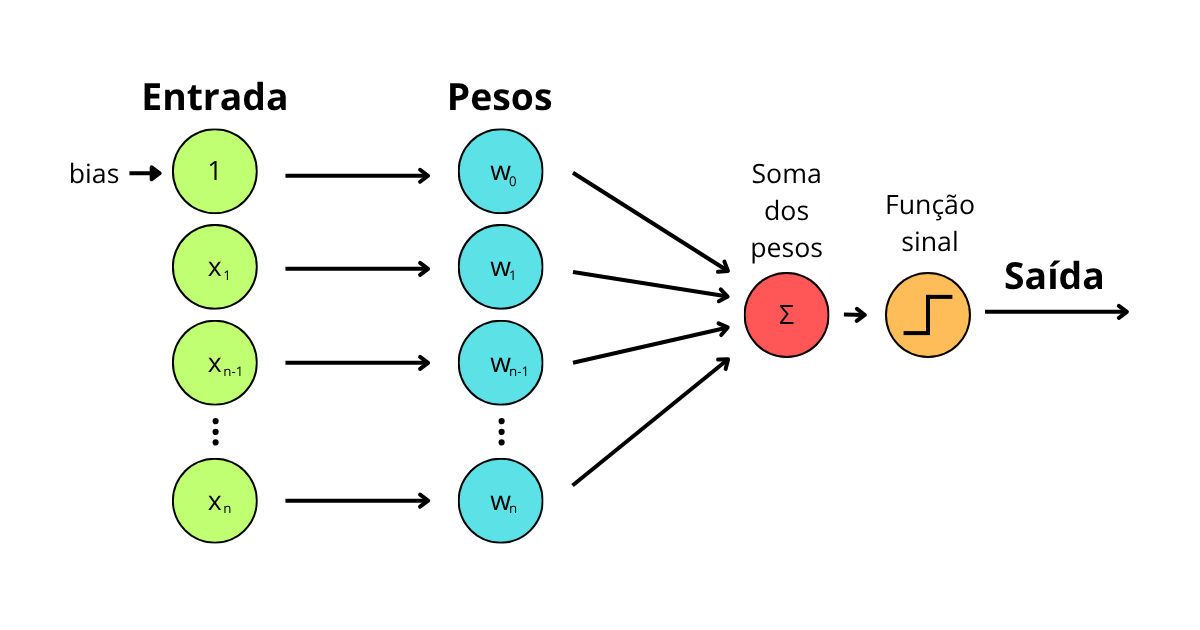
\includegraphics[width=1.0\textwidth]{images/perceptron.png}
	
	\vspace{5pt} % Espaçamento sutil entre a imagem e a fonte
	\centering
	\small Fonte: Elaborado pelo autor (2026).
\end{figure}

Um perceptron linear isolado não representa relações não lineares. A combinação de unidades em camadas ocultas, com funções de ativação não lineares, permite às redes neurais representar relações que esse classificador não consegue capturar. Nesse contexto, desenvolve-se a arquitetura de redes com múltiplas unidades e camadas.

Na descrição de \citeonline{ghosh2023machine}, a rede reúne unidades conectadas por pesos ajustáveis. Para compreender o treinamento de redes multicamadas, é necessário introduzir a retropropagação, também denominada \textit{backpropagation}.

O perceptron de \citeonline{rosenblatt1958perceptron} classifica padrões linearmente separáveis. Suas entradas são multiplicadas pelos respectivos pesos, somadas ao viés e submetidas a uma função sinal ou degrau\footnote{As funções diferem no tratamento do ponto zero, mas ambas produzem uma decisão discreta e não são diferenciáveis nesse ponto.}. Durante o treinamento, os pesos são atualizados quando a saída prevista difere da saída esperada.

A limitação pode ser observada no problema do ou exclusivo (XOR), exemplo clássico de classificação não linearmente separável. Quando as entradas binárias são diferentes, o resultado é 1; quando são iguais, o resultado é 0, conforme a tabela verdade:

\begin{table}[htb]
	\centering
	\captionsetup{justification=centering}
	\caption{Tabela verdade da operação XOR}
	\label{tab:xor}
	\begin{tabular}{ccc}
		\hline
		A & B & $A \oplus B$ \\
		\hline
		0 & 0 & 0 \\
		0 & 1 & 1 \\
		1 & 0 & 1 \\
		1 & 1 & 0 \\
		\hline
	\end{tabular}
	\\[0.2cm]
	\footnotesize Fonte: Elaborado pelo autor (2026).
\end{table}

\citeonline{minsky1969introduction} discutem a limitação do perceptron de \citeonline{rosenblatt1958perceptron} diante de problemas que não são linearmente separáveis, como o XOR. Em uma representação gráfica, uma única reta não separa corretamente suas classes. A repercussão dessa limitação é frequentemente associada ao período posteriormente denominado "inverno da IA".

O desenvolvimento de redes multicamadas ganhou impulso com a difusão da retropropagação. \citeonline{rumelhart1986learning} descrevem sua aplicação ao ajuste dos pesos das conexões: "O procedimento ajusta repetidamente os pesos das conexões na rede para minimizar uma medida da diferença entre o vetor de saída real da rede e o vetor de saída desejado." \citem[p. 533, tradução nossa]{rumelhart1986learning}.

As redes apresentadas por \citeonline{rumelhart1986learning} empregam uma arquitetura \textit{feedforward}, na qual os dados fluem da entrada para a saída. Nas camadas totalmente conectadas, cada unidade de uma camada se liga às unidades da camada seguinte.

O treinamento por retropropagação exige funções de ativação que permitam o cálculo dos gradientes utilizados no ajuste dos pesos. A função sinal do perceptron de \citeonline{rosenblatt1958perceptron} não é diferenciável no ponto de descontinuidade e, por isso, é substituída no treinamento de redes multicamadas por funções adequadas à otimização por gradiente. Um exemplo é a função sigmoide\footnote{Outras funções de ativação incluem ReLU (unidade linear retificada), tangente hiperbólica, Softmax e função linear. A escolha da ativação, do número de camadas e da taxa de aprendizagem integra a definição dos hiperparâmetros do modelo e pode afetar seu desempenho.}, representada na equação \ref{eq:sigmoide} e na figura \ref{fig:sigmoide}.

\begin{equation}
	\label{eq:sigmoide}
	f(x) = \dfrac{1}{1 + e^{-x}}
\end{equation}

\begin{figure}[h]
	\captionsetup{justification=centering}
	\caption{Função Sigmoide}
	\label{fig:sigmoide}
	\vspace{5pt}
	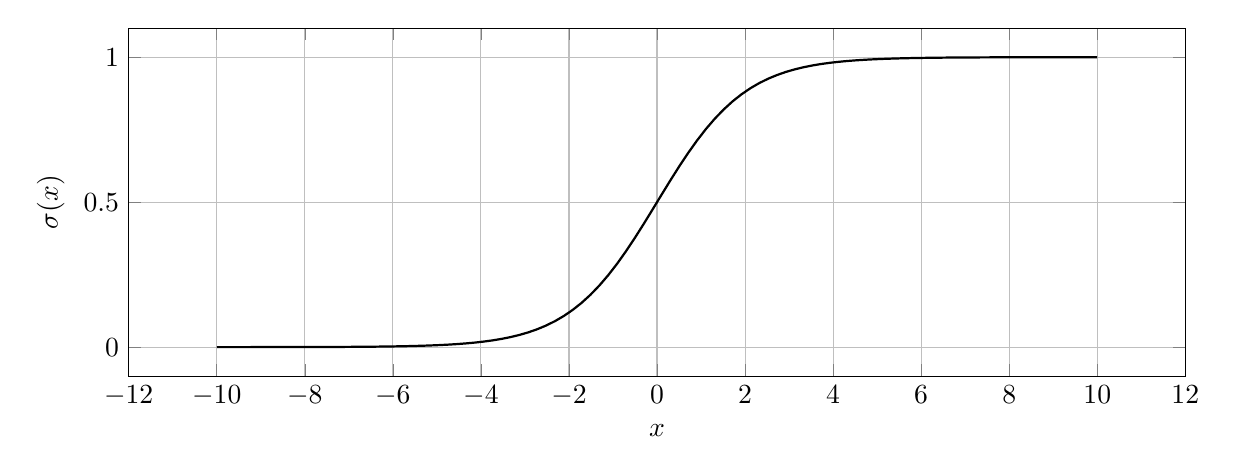
\begin{tikzpicture}
		\begin{axis}[
			xlabel={$x$},
			ylabel={$\sigma(x)$},
			domain=-10:10,
			samples=100,
			grid=major,
			width=15cm,
			height=6cm
			]
			\addplot[thick] {1/(1+exp(-x))};
		\end{axis}
	\end{tikzpicture}
	\vspace{5pt}
	\centering
	\small Fonte: Elaborado pelo autor (2026).
\end{figure}

Nas redes multicamadas, o erro observado na saída orienta o ajuste dos pesos das camadas anteriores. A retropropagação transmite a informação necessária ao ajuste de uma camada à anterior, sucessivamente. Esse procedimento é repetido durante o treinamento para reduzir a função de erro.

O ajuste dos pesos utiliza derivadas da função de erro. A derivada mede a variação local de uma função em relação a uma variável e, geometricamente, corresponde à inclinação da reta tangente à curva em um ponto.

Para ilustrar esse processo, considere a função de erro quadrático apresentada na equação \ref{eq:mse}:

\begin{equation}
	E = \frac{1}{2}(y-\hat{y})^2
	\label{eq:mse}
\end{equation}

Onde:
\begin{itemize}
	\item $y$ representa o valor observado;
	\item $\hat{y}$ representa o valor predito;
	\item $E$ representa o erro quadrático.
\end{itemize}

A função está representada na figura \ref{fig:erroquadratico}.

\begin{figure}[htb]
	\centering
	\captionsetup{justification=centering}
	\caption{Função de erro quadrático}
	\vspace{5pt}
	\label{fig:erroquadratico}
	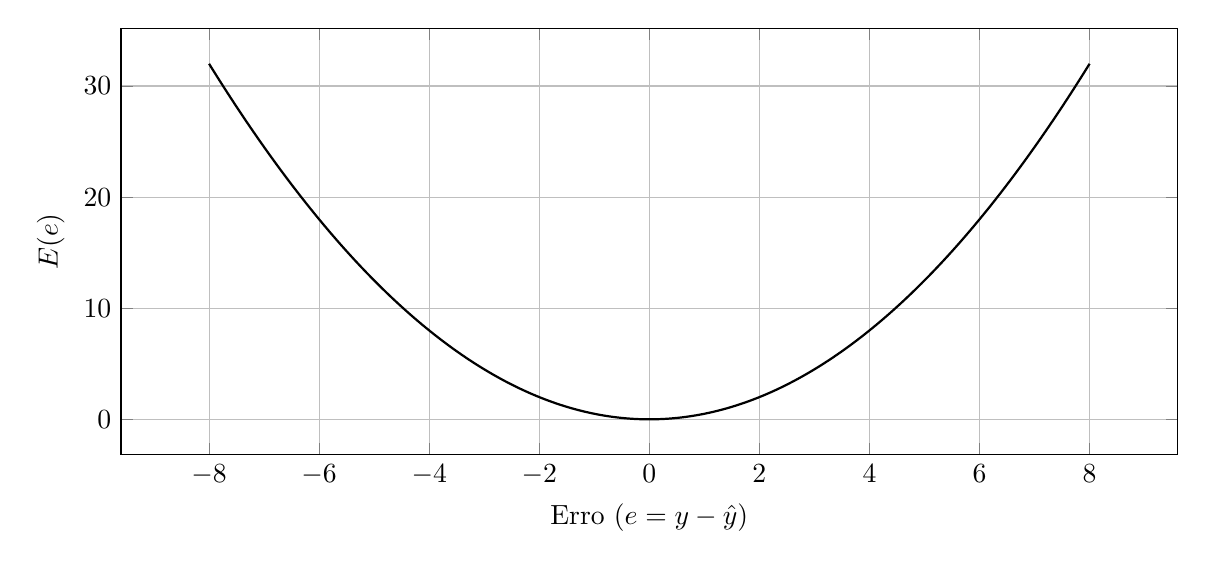
\begin{tikzpicture}
		\begin{axis}[
			xlabel={Erro ($e=y-\hat{y}$)},
			ylabel={$E(e)$},
			domain=-8:8,
			samples=200,
			grid=major,
			width=15cm,
			height=7cm
			]
			\addplot[thick] {0.5*x^2};
		\end{axis}
	\end{tikzpicture}

	\vspace{0.2cm}
	\footnotesize Fonte: Elaborado pelo autor (2026).
\end{figure}

A derivada indica a direção de variação local da função de erro. No treinamento, essa informação orienta o ajuste dos parâmetros do modelo para reduzir o erro, como ilustra a figura \ref{fig:gradiente_descendente_erro}.

\begin{figure}[htb]
	\centering
	\captionsetup{justification=centering}
	\caption{Função de erro quadrático e segmentos de retas tangentes representando a derivada em diferentes pontos}
	\vspace{5pt}
	\label{fig:gradiente_descendente_erro}
	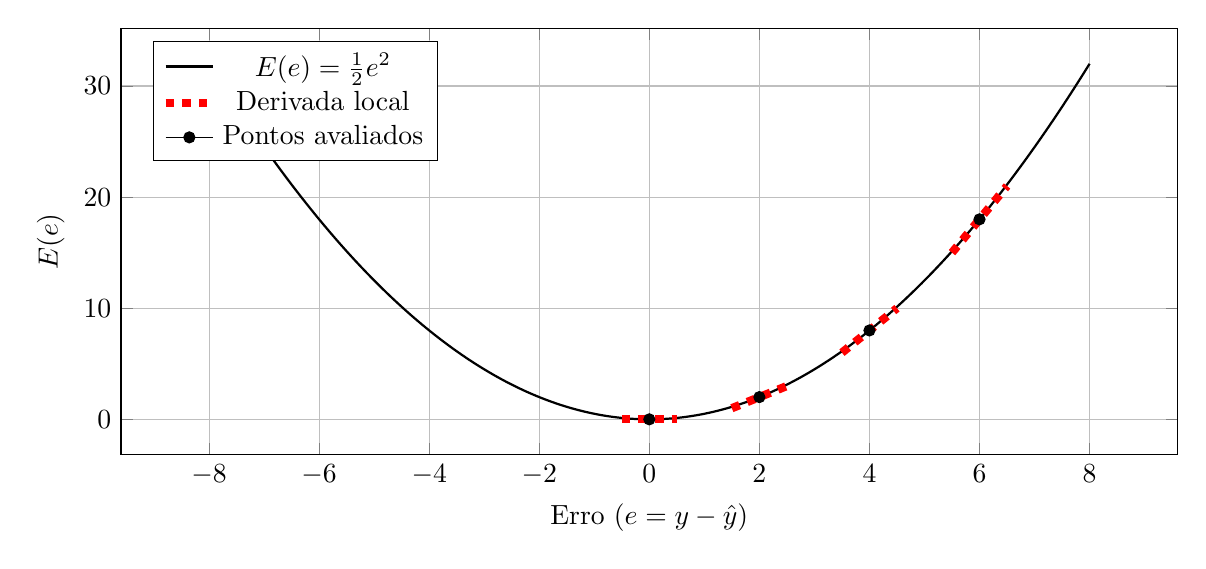
\begin{tikzpicture}
		\begin{axis}[
			xlabel={Erro ($e=y-\hat{y}$)},
			ylabel={$E(e)$},
			grid=major,
			width=15cm,
			height=7cm,
			legend pos=north west
			]
			
			% Função de erro
			\addplot[
			thick,
			domain=-8:8,
			samples=200
			] {0.5*x^2};
			\addlegendentry{$E(e)=\frac{1}{2}e^2$}
			
			% Ponto e=6
			\addplot[dashed, color=red, line width=3pt, domain=5.5:6.5] {6*(x-6)+18};
			\addlegendentry{Derivada local}
			\addplot[mark=*] coordinates {(6,18)};
			\addlegendentry{Pontos avaliados}
			
			% Ponto e=4
			\addplot[dashed, color=red, line width=3pt, domain=3.5:4.5] {4*(x-4)+8};
			\addplot[mark=*] coordinates {(4,8)};
			
			% Ponto e=2
			\addplot[dashed, color=red, line width=3pt, domain=1.5:2.5] {2*(x-2)+2};
			\addplot[mark=*] coordinates {(2,2)};
			
			% Ponto e=0
			\addplot[dashed, color=red, line width=3pt, domain=-0.5:0.5] {0};
			\addplot[mark=*] coordinates {(0,0)};
			
		\end{axis}
	\end{tikzpicture}

	
	\vspace{0.2cm}
	\footnotesize Fonte: Elaborado pelo autor (2026).
\end{figure}

Em uma rede neural, a função de erro pode ter muitos parâmetros e uma superfície mais complexa do que a função quadrática usada no exemplo. A figura \ref{fig:superficie_erro} ilustra uma superfície em duas dimensões, suficiente para introduzir a ideia de gradiente descendente, embora não represente toda a complexidade de uma rede profunda.

\begin{figure}[htb]
	\centering
	\captionsetup{justification=centering}
	\caption{Superfície de erro}
	\label{fig:superficie_erro}
	\vspace{5pt}
	
	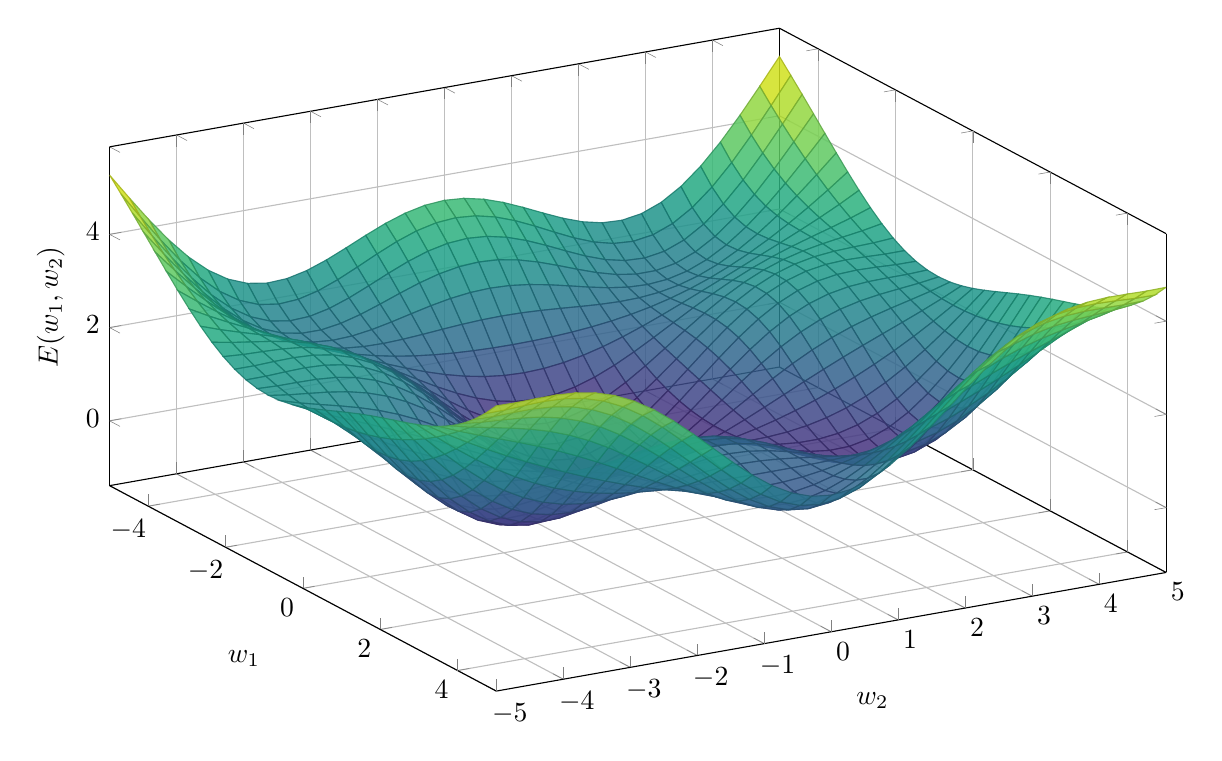
\begin{tikzpicture}
		\begin{axis}[
			view={60}{35},
			width=15cm,
			height=10cm,
			xlabel={$w_1$},
			ylabel={$w_2$},
			zlabel={$E(w_1,w_2)$},
			colormap/viridis,
			grid=major
			]
			
			% Superfície de erro
			\addplot3[
			surf,
			opacity=0.85,
			samples=35,
			domain=-5:5,
			y domain=-5:5
			]
			{0.1*(x^2+y^2)+sin(deg(x))*cos(deg(y))};
			
		\end{axis}
	\end{tikzpicture}
	

	\vspace{0.2cm}
	\footnotesize Fonte: Elaborado pelo autor (2026).
	
\end{figure}

O gradiente descendente "É um método iterativo no qual começamos com um palpite inicial da solução e depois refinamos gradualmente." \citem[p. 45, tradução nossa]{ekman2021learning}. Em uma função de uma variável, a derivada orienta os ajustes sucessivos. Para funções de várias variáveis, utiliza-se o gradiente:

\begin{citacao}
	Se tivermos uma função de n variáveis, então nosso gradiente consistirá em n derivadas parciais, e podemos calcular o próximo passo como $x-\eta \nabla y$, onde tanto $x$ quanto $\nabla y$ são vetores com $n$ elementos.  \citem[p. 47, tradução nossa]{ekman2021learning}
\end{citacao}

Uma analogia ajuda a visualizar o gradiente descendente: um animal cego e com sede percorre um terreno acidentado em busca de água nos vales. Sem conhecer a posição da água, ele percebe a inclinação do solo e segue, a cada passo, a direção de descida.

A analogia também ilustra a possibilidade de convergência para mínimos locais: uma depressão do terreno pode parecer o ponto mais baixo em sua vizinhança, embora não corresponda ao mínimo global da superfície. De modo semelhante, o gradiente descendente pode alcançar uma solução local, dependendo da função de erro, da inicialização e dos parâmetros de treinamento\footnote{Para uma discussão mais ampla sobre funções de ativação, taxa de aprendizagem, gradiente descendente e estratégias de otimização, consulte \citeonline{ekman2021learning}.}.

% Ainda estou pensando se coloco a parte de algebra linear no texto para falar sobre a formulação matemática, vou perguntar para o professor

O aprendizado profundo (\textit{deep learning}) utiliza redes neurais com múltiplas camadas de representação. A distinção em relação a redes menos profundas não decorre de um limite universal de camadas, mas da maior profundidade da arquitetura e de sua capacidade de representar padrões complexos. Essa ampliação também aumenta a importância de avaliar problemas como sobreajuste, otimização e interpretabilidade.

Na previsão econômica, a escolha de uma rede neural deve considerar simultaneamente o erro de previsão e a possibilidade de interpretar o resultado para a decisão em análise. A arquitetura mais adequada depende, portanto, dos objetivos da aplicação e do equilíbrio pretendido entre desempenho preditivo e interpretabilidade.

Após essa apresentação simplificada\footnote{A formulação completa das redes neurais envolve conceitos de otimização e álgebra linear que excedem o nível de detalhe adotado nesta monografia. Para uma exposição matemática mais aprofundada, consulte \citeonline{ekman2021learning}.} dos princípios das redes neurais, examinamos suas aplicações à previsão econômica.

\citeonline{vasconcelos2017poder} utiliza redes neurais em uma tese baseada em dados de 41 países, em geral de 2001 a 2015. A amostra reúne principalmente membros da \ac{ocde}, além de outros países escolhidos por sua relevância econômica ou pela disponibilidade de dados. Segundo o autor, algumas séries abrangem períodos mais longos.

O autor reúne variáveis trimestrais relativas ao PIB e seus componentes, comércio internacional, preços, câmbio, juros, títulos públicos, mercados financeiros, crédito e preços de commodities. Entre os indicadores financeiros estão CDS\footnote{\textit{Credit Default Swap}, indicador associado ao risco de crédito.} e VIX\footnote{Índice de volatilidade.}. As séries\footnote{Para mais detalhes sobre as variáveis, consulte \citeonline{vasconcelos2017poder}.} foram obtidas em bases como Banco Mundial, \ac{ocde}, BIS e Bloomberg.

O autor compara modelos de equações individuais, fatores comuns, modelos mistos estimados por mínimos quadrados ordinários, Lasso, regressão em árvore e métodos de \textit{machine learning}, como \textit{Support Vector Machine}, \textit{Random Forest} e \textit{deep learning}.

O autor investigou as relações entre política fiscal, mercado internacional e flutuações do produto. Em termos preditivos, os modelos de \textit{deep learning} superaram os modelos de equações individuais e de fatores comuns, mas tiveram desempenho inferior ao dos modelos mistos e de outros métodos de \textit{machine learning} analisados na tese.

Na análise das relações econômicas, os modelos apontaram maior relevância do mercado internacional do que da política fiscal. O autor também destaca a utilidade das redes neurais para a previsão macroeconômica, embora os resultados indiquem que seu desempenho varia conforme o método de comparação e a aplicação considerada.

\citeonline{carmo2023modelagem} comparam regressão linear simples e redes neurais multicamadas, classificadas no estudo como métodos clássico e contemporâneo, respectivamente. Os modelos foram aplicados à previsão da remuneração média mensal dos empregados nas 27 unidades da federação, com dados do \ac{ibge} obtidos pelo \ac{sidra}. No critério de precisão utilizado pelos autores, as redes neurais tiveram melhor desempenho. O estudo também aponta limitações de interpretabilidade dessas redes, tema discutido por \citeonline{vasconcelos2017poder}.

\begin{citacao}
	Do ponto de vista analítico, a análise de regressão linear é mais dinâmica e informativa que a RNA MLP\footnote{Redes Neurais Artificiais \textit{Multilayer Perceptron}}. Pois, ao identificar os coeficientes do modelo de regressão e seus sinais, é possível compreender o impacto de cada variável independente significativa na explicação do comportamento da variável de estudo. Ao passo que, a RNA MLP somente permite avaliar qual o grau de importância das variáveis  explicativas do modelo. \citem[p. 17]{carmo2023modelagem}
\end{citacao}

Nesse estudo, o desempenho das redes neurais variou conforme o método de comparação. A seleção de variáveis em uma regressão depende do procedimento adotado e não constitui uma limitação intrínseca dos modelos lineares. As redes neurais, por sua vez, permitem representar relações não lineares, característica relevante para a comparação realizada pelos autores.

Os autores assinalam vantagens e limitações nas duas abordagens. A regressão linear favorece a interpretação dos coeficientes, enquanto as redes neurais oferecem maior flexibilidade para representar relações não lineares. Essa flexibilidade, entretanto, é acompanhada por maior complexidade arquitetural e menor interpretabilidade direta.

\citeonline{amaral2023previsao} comparam diferentes configurações de redes neurais. Enquanto as arquiteturas apresentadas anteriormente são totalmente conectadas e do tipo \textit{feedforward}, os três modelos avaliados por \citeonline{amaral2023previsao} são baseados em \ac{rnn}.

\begin{citacao}
	As \ac{rnn} são um tipo de rede neural que foi 
	desenvolvida para identificar padrões em um banco de dados. Através dos algoritmos da rede neural, ele é capaz de identificar, dentro de uma sequência de informações, similaridades de palavras, de texto, imagens e números, utilizando esses padrões para aprender e futuramente entender o que o está sendo “apresentado”. \citem[p. 11]{amaral2023previsao}
\end{citacao}

Além disso, os autores utilizaram uma arquitetura de rede neural recorrente denominada \ac{lstm}, projetada para representar dependências em sequências. Essa característica a torna pertinente à análise de séries temporais, nas quais podem coexistir padrões de diferentes horizontes.

Os autores testaram três configurações: univariada \textit{stacked}\footnote{Esse modelo "possui uma arquitetura de mais de uma camada de neurônio escondida, no qual cada camada contém múltiplas células de memória" \citem[p. 13]{amaral2023previsao}.}, multivariada e univariada bidirecional\footnote{Na configuração bidirecional, uma rede processa a sequência na ordem original e outra, na ordem inversa \citem{amaral2023previsao}.}. Os dados foram obtidos no Banco Central do Brasil e no \ac{ibge}, abrangendo o período de janeiro de 2002 a março de 2023. O conjunto inclui taxa \ac{selic}, \ac{ipca}, \ac{pim} e taxa de câmbio.

Entre as três configurações de redes \ac{lstm}, o modelo multivariado apresentou os menores erros; esse resultado, por si só, não permite concluir que tenha maior interpretabilidade. O segundo melhor desempenho foi obtido pelo modelo univariado \textit{stacked}, especialmente nas especificações que utilizaram a taxa \ac{selic} como entrada. O modelo univariado bidirecional não superou o modelo univariado \textit{stacked} em nenhuma das variáveis analisadas.

Os autores observam que o modelo multivariado teve desempenho satisfatório mesmo com uma quantidade limitada de dados. Ressaltam, contudo, a importância de que profissionais da área também considerem indicadores históricos e informações contextuais na análise.

O estudo de \citeonline{amaral2023previsao} apresenta uma aplicação de redes recorrentes a séries econômicas e mostra que o desempenho varia entre configurações. A avaliação desses resultados também requer atenção à interpretabilidade e ao contexto econômico.

Na literatura internacional, \citeonline{ghosh2023machine} examinam o uso de redes neurais para a previsão do \ac{gdp} da Índia com dados de janeiro de 2003 a dezembro de 2019. O estudo é pertinente aqui por aplicar modelos de previsão a uma variável macroeconômica, embora o país, a frequência dos dados e o desenho da pesquisa sejam distintos dos deste trabalho.

Os autores utilizaram 13 indicadores, além do \ac{gdp}, com dados do Banco da Reserva da Índia e da CEIC\footnote{Base de dados de indicadores macroeconômicos globais.}. A estrutura combina um \ac{dfm}, que sintetiza as informações dos indicadores, com modelos empregados para gerar previsões desses indicadores, entre eles \textit{Random Forest}, ARIMA e Prophet. Em seguida, uma equação-ponte relaciona os fatores estimados ao \ac{gdp}, utilizando especificações com AR(1) ou redes neurais. O estudo integra, portanto, componentes de previsão em frequências distintas no exercício de \textit{nowcasting}.

Nos resultados reportados, a combinação do Prophet para a previsão dos indicadores com redes neurais na equação-ponte apresentou o melhor desempenho dentro da amostra. Para horizontes mais longos, o erro aumentou, o que limita a extrapolação dos resultados de \textit{nowcasting} para previsões de longo prazo.

O estudo de \citeonline{ghosh2023machine} difere deste trabalho pelo foco em \textit{nowcasting} e pela combinação de séries de diferentes frequências. Sua contribuição para esta revisão está em ilustrar como redes neurais podem integrar uma estrutura composta por DFM, modelos de previsão dos indicadores e uma equação-ponte para o PIB.

Os estudos examinados mostram diferentes aplicações de redes neurais à previsão econômica. Sua flexibilidade permite representar relações não lineares, mas a especificação, o treinamento e a interpretação continuam dependendo das escolhas do pesquisador, como discutem \citeonline{carmo2023modelagem} e \citeonline{amaral2023previsao}.

Em relação ao perceptron de \citeonline{rosenblatt1958perceptron}, as aplicações atuais utilizam arquiteturas mais amplas e podem combinar redes neurais com outros métodos. Os resultados de \citeonline{amaral2023previsao} e \citeonline{ghosh2023machine} mostram, contudo, que o desempenho depende da configuração e do horizonte de previsão, o que reforça a necessidade de avaliação empírica para cada problema.

 

\subsubsection{Random Forest}

O último modelo examinado nesta revisão é o \textit{Random Forest}, ou floresta aleatória. Sua apresentação complementa a discussão dos métodos baseados em IA utilizados neste trabalho.

\citeonline{breiman2001random} apresenta o \textit{Random Forest} como uma "combinação de preditores em forma de árvore, de modo que cada árvore depende dos valores de um vetor aleatório amostrado de forma independente e com a mesma distribuição para todas as árvores da floresta." \citem[p. 1, tradução nossa]{breiman2001random}. Na aplicação à regressão, o método combina as previsões das árvores pela média de seus resultados.

Para tarefas de classificação, \citeonline{breiman2001random} apresenta a seguinte definição:

\begin{citacao}
	É um classificador que consiste em uma coleção de classificadores em forma de árvore $\{h(\mathbf{x}, \theta_k), k=1, ... \}$, onde os $\{k\}$ são vetores aleatórios independentes e identicamente distribuídos, e cada árvore dá um voto unitário para a classe mais popular na entrada $\mathbf{x}$. \citem[p. 6, tradução nossa]{breiman2001random}
\end{citacao}

Na regressão com \textit{Random Forest}\footnote{Em tarefas de classificação, as árvores votam nas classes possíveis, e a classe mais votada constitui a resposta da floresta.}, a previsão final corresponde à média das previsões das árvores. \citeonline{landowska2025gdpgfcfdynamicsglobaleconomies} descreve a agregação dos resultados e observa que o método "constrói múltiplas árvores de decisão e agrega seus resultados, o que lhe permite lidar com conjuntos de dados de alta dimensão, reduzir o overfitting e fornecer insights valiosos sobre a importância das variáveis." \citem[p. 5]{landowska2025gdpgfcfdynamicsglobaleconomies}.

\citeonline{lemos2025atas} explica que o \textit{Random Forest} pode utilizar árvores de regressão, um tipo de árvore de decisão. Nesse caso, "cada nó representa uma condição de decisão baseada em uma variável preditora, fornecendo um valor numérico, que normalmente é a média dos valores observados nas amostras que atingem aquele nó." \citem[p. 8]{lemos2025atas}. \citeonline{landowska2025gdpgfcfdynamicsglobaleconomies} destaca a capacidade do método de representar relações não lineares e interações entre variáveis.

A equação \ref{eq:random_forest} representa a previsão da floresta como a média das previsões de suas $B$ árvores, conforme a descrição de \citeonline{vasconcelos2017poder}.

\begin{equation}
	\label{eq:random_forest}
	\hat f_{\mathrm{floresta}}(X) = \frac{1}{B}\sum_{b=1}^{B} f_b(X)
\end{equation}

%oferece vantagens significativas em relação aos modelos econométricos tradicionais, principalmente na sua capacidade de lidar com relações não lineares e interações entre variáveis

O \textit{Random Forest} aparece em diferentes aplicações econômicas: \citeonline{landowska2025gdpgfcfdynamicsglobaleconomies} o emprega na previsão do \ac{gdp}; \citeonline{lemos2025atas} utiliza informações de atas do COPOM; e \citeonline{kava2022alem} o inclui entre os modelos candidatos à previsão de variáveis macroeconômicas brasileiras.

Além da importância das variáveis, a interpretação do \textit{Random Forest} pode recorrer a funções de dependência parcial. Conforme \citeonline{rebelo2022interpretabilidade}, essas funções mostram o efeito marginal de um ou dois preditores sobre a previsão do modelo. Os gráficos descrevem como a previsão média varia ao longo dos valores do preditor analisado. Essa leitura é associativa: representa o comportamento estimado pelo modelo e, isoladamente, não demonstra uma relação causal entre a variável e o PIB.

O conjunto de modelos apresentado delimita as abordagens comparadas neste trabalho. As diferenças de estrutura, quantidade de variáveis, frequência dos dados e possibilidade de interpretação fornecem a base para a metodologia e para a análise dos resultados. Nos capítulos seguintes, a comparação considera o tempo de execução, a interpretabilidade qualitativa e o desempenho preditivo medido por RMSE e MAE, tendo como alvos o crescimento e o nível anual do PIB real brasileiro.

%\citeonline{kava2022alem} e de \citeonline{rebelo2022interpretabilidade} que

%Diante desse contexto optamos por apresentar os modelos de uma maneira didática, do mais "fácil" ao mais "difícil", isso é um juízo de valor bem subjetivo, contudo para construção de uma sequência lógica possível de acompanhar, descrever os modelos em grau de complexidade, parece ser uma boa alternativa para um texto compreensível.
%
%Certamente o grau de complexidade de um modelo está relacionado a quantidade de variáveis usadas, assim como o quão trabalhoso é para se aplicar esse modelo, nesse sentido o ARIMA, talvez seja um dos modelos preditivos mais simples.

%O ARIMA, ou em português, modelo auto-regressivo de médias móveis, é um modelo que utiliza da pr

% EU QUERO COLOCAR OS TESTES, MAS SE NÃO DER TEMPO NÃO COLOCAREI NA QUALIFICAÇÃO

%\section{Testes: Comprovar e comparar modelos}
%\label{sec:testes}

%	\citem{laudon2022sistemas} sistemas de informação são essenciais para alcançar objetivos estratégicos dos negócios. Na era digital, o grande volume de dados gerados pelos sistemas de informação pode ser usada como uma fonte, praticamente inesgotável de informações para tomadas de decisões. 
%
%	Rever trabalhos sobre uso dessas técnicas para predição

% NÃO SEI SE IREI COLOCAR ESSA SESSÃO, MAS PENSO QUE SIM
%\section{IA vs Tradicional: Uma perspectiva Acadêmica}
